% main.tex
\documentclass{article}

\usepackage[pdfauthor={CoderDojo Linz},
            pdftitle={Feuerwerk in TypeScript}]
            {hyperref}



\newcommand{\footertitle}{Bubble sorter in Scratch}
% settings.tex
\usepackage[
    a4paper, 
    top=2cm,
    left=1cm,
    right=1cm,
    bottom=2cm
]{geometry}

\usepackage{fontspec}
\usepackage{graphicx}
\usepackage{hyperref}
\usepackage{fancyhdr}
\usepackage[ngerman]{babel}
\usepackage{wrapfig}
\usepackage{enumitem}
\usepackage{titlesec} 
\usepackage{ragged2e}
\usepackage{tcolorbox}
\usepackage{array}
\usepackage[table]{xcolor}
\usepackage{fontawesome5}

\setmainfont{Carlito}

% Fancyhdr setup
\fancypagestyle{defaultpagestyle}{
    \fancyhf{} % Clear all headers and footers
    \fancyhead[C]{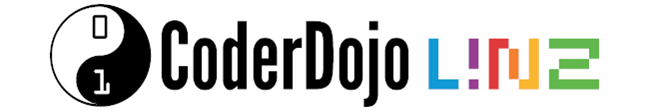
\includegraphics[width=5cm]{../../CoderDojo_Logo.png}} 
    \renewcommand{\headrulewidth}{0pt} % Remove header line
    \renewcommand{\footrulewidth}{0pt} % Remove footer line
    \fancyfoot[L]{\footertitle}
    \fancyfoot[R]{Seite \thepage} % Right footer with page number
}

\newcommand{\SectionDesign}[4]{
    \noindent
    \csname #1*\endcsname{\textcolor[HTML]{1E90FF}{\fontsize{#2pt}{#3pt}\selectfont #4}}
}

\newcommand{\TextAndImage}[5][{}]{
    \fontsize{11pt}{16pt}\selectfont
    \noindent
    \begin{minipage}[c]{#4\textwidth}
    \RaggedRight
    #2 % First parameter: text
    \end{minipage}
    \hfill
    \begin{minipage}[c]{#5\textwidth}
    \includegraphics[width=\textwidth, #1]{#3} % Second parameter: image file name
    \end{minipage}
}

\newcommand{\ImageAndText}[2]{
    \fontsize{16pt}{24pt}\selectfont
    \noindent
    \begin{minipage}[c]{0.65\textwidth}
        \includegraphics[width=\textwidth]{#1} % Second parameter: image file name
    \end{minipage}
    \hfill % Fills the space between the minipages
    \begin{minipage}[c]{0.25\textwidth}
        \centering
        #2 % First parameter: text
    \end{minipage}
}

\newcommand{\TextDesign}[1]{
    \fontsize{11pt}{16pt}\selectfont
    \noindent
    \RaggedRight
    #1 % First parameter: text
}
\graphicspath{{images/}}

\begin{document}
    \pagestyle{defaultpagestyle}

    \SectionDesign{section}{24}{24}{\textbf{Bubble Sorter mit Scratch}}
    \vspace{1cm}
     
    \ImageAndText{MainPic.png}{
    \centering
    Heute programmieren wir eine herausfordende Scratch Übung namens Bubble Sorter. Hierbei kannst du deine Scratch Kentnisse verbessern.
    }{0.6}{0.3}{16}{24}
    
    \vspace{2cm}
    \SectionDesign{subsection}{18}{24}{\textbf{Ziel der Übung}}
    \vspace{0.5cm}

    \TextDesign{
    Heute wollen wir gemeinsam einen Bubble sorter basteln, hierbei geht es darum den Algorhytmus zu verstehen, mit Klonen zu Arbeiten und dich selber etwas heraus zu fordern.

    \vspace{\baselineskip}
    Du solltest für diese Übung schon ein wenig Programmiererfahrung mit einer Blockprogrammiersprache wie \textit{Scratch} oder \textit{Snap!} haben. 
    }

    \vspace{1cm}
    \SectionDesign{subsection}{18}{24}{\textbf{Start}}
    \vspace{0.5cm}

    \TextDesign{
    Du brauchst für diese Übung keine spezielle Software auf deinem Computer zu installieren. Scratch kannst du auch im Web-browser verwenden. Um los zu legen müssen wir als erstes unsere Figuren und den Hintergrund fest legen. Wir brauchen dafür Bälle und natürlich ein Gefäß für unsere Bälle. Eine Figur die mit dem Benutzer spricht und einen schönen Hintergrund.}

     % NEWPAGE
    \newpage
    
    \vspace{0.5cm}
    
    \SectionDesign{subsection}{18}{24}{\textbf{Hintergrund festlegen und zuschneiden}}
    \vspace{1cm}
     
    \ImageAndText{HintergrundBild.png}{
    
  Das hier wird der Hintergrund für unser Spiel ich werde dir gleich Zeigen wie man ihn einbindet in Scratch. 
    }{0.6}{0.3}{12}{24}
    
\vspace{1cm}
    \TextDesign{
    Als erstes schauen wir uns dafür unseren Start Bildschirm an wenn wir ein neues Projekt anlegen. Wenn du noch nichst verändert hast und deine Sprache auf Deutsch eingestellt ist sollte dein Startbildschirm so aussehen: 
    } 
    \vspace{0.5cm}
    
    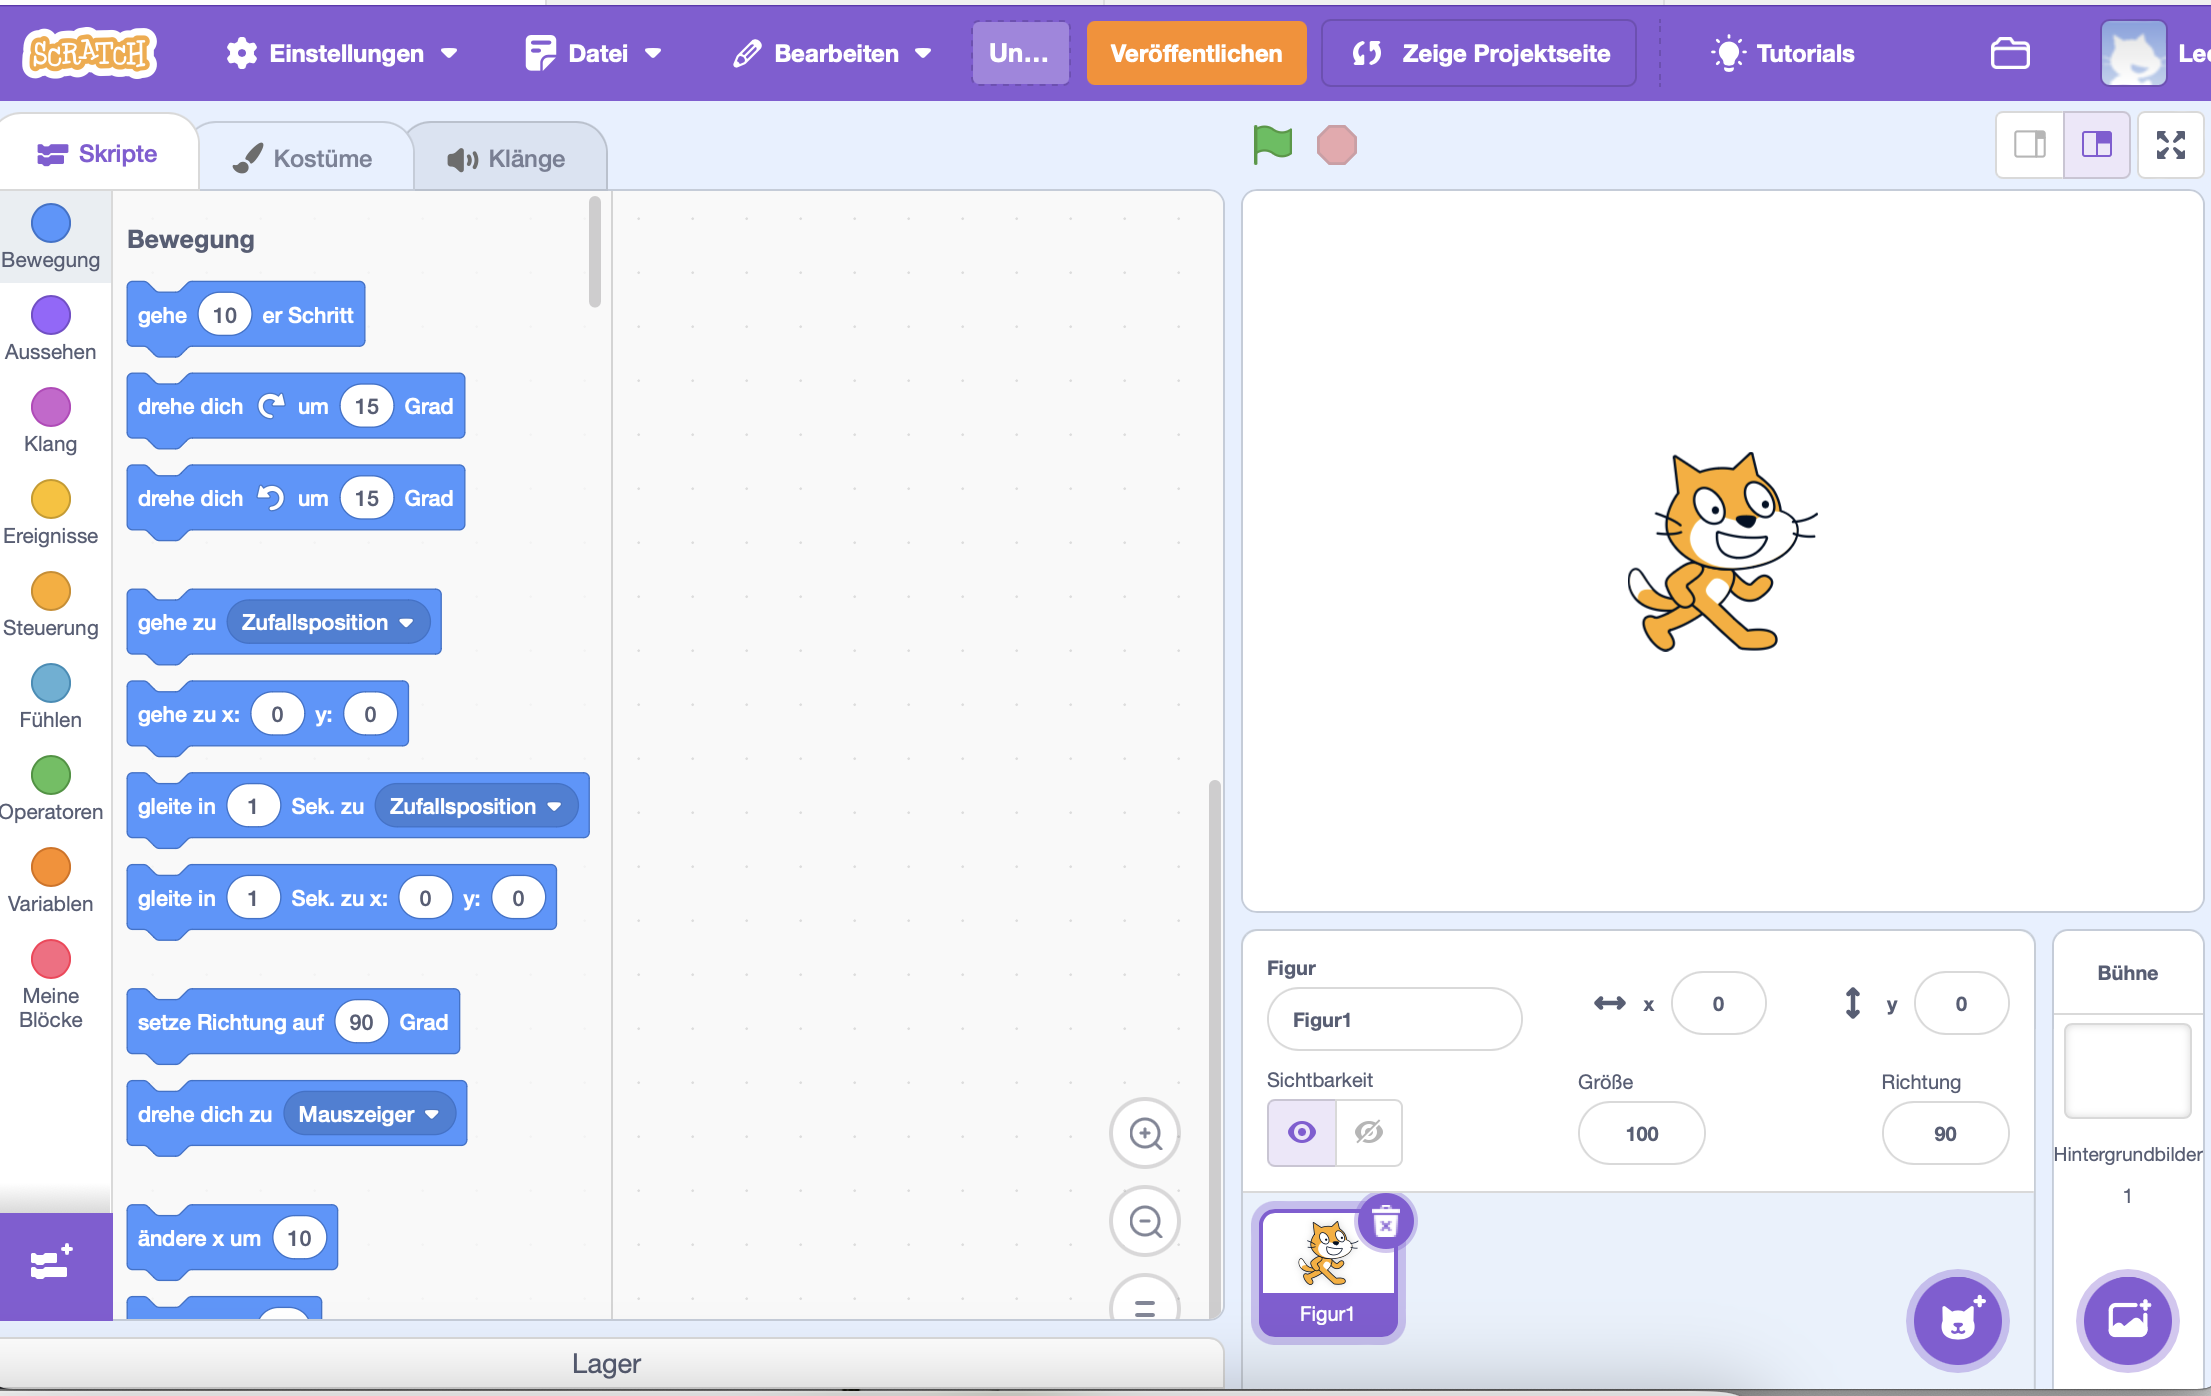
\includegraphics[width=0.8\textwidth, height=9cm]{Startbildschrim.png}

\TextAndImage{
    Wenn du auf das grüne Zeichen ganz unten auf der rechten Seite deines Bildschirmes klickst solltest du dieses Menü sehen. Um unseren eigenen Hintergrund hinzu zu fügen müssen wir ihn als erstes hochladen. Das machen wir mit den ganz obersten Zeichen (das mit dem Pfeil). Wenn du drauf klickst öffnen sich automatisch deine Datein jetzt musst du nur noch das richtige Bild auswählen und "Hochladen" klicken.
}{ZeichenH.png}{0.4}{0.15}{11}{16}

\vspace{1cm}
    \TextDesign{
    Jetzt sollte dein Bildschirm automatisch so aussehen:
    } 
    \vspace{0.4cm}

    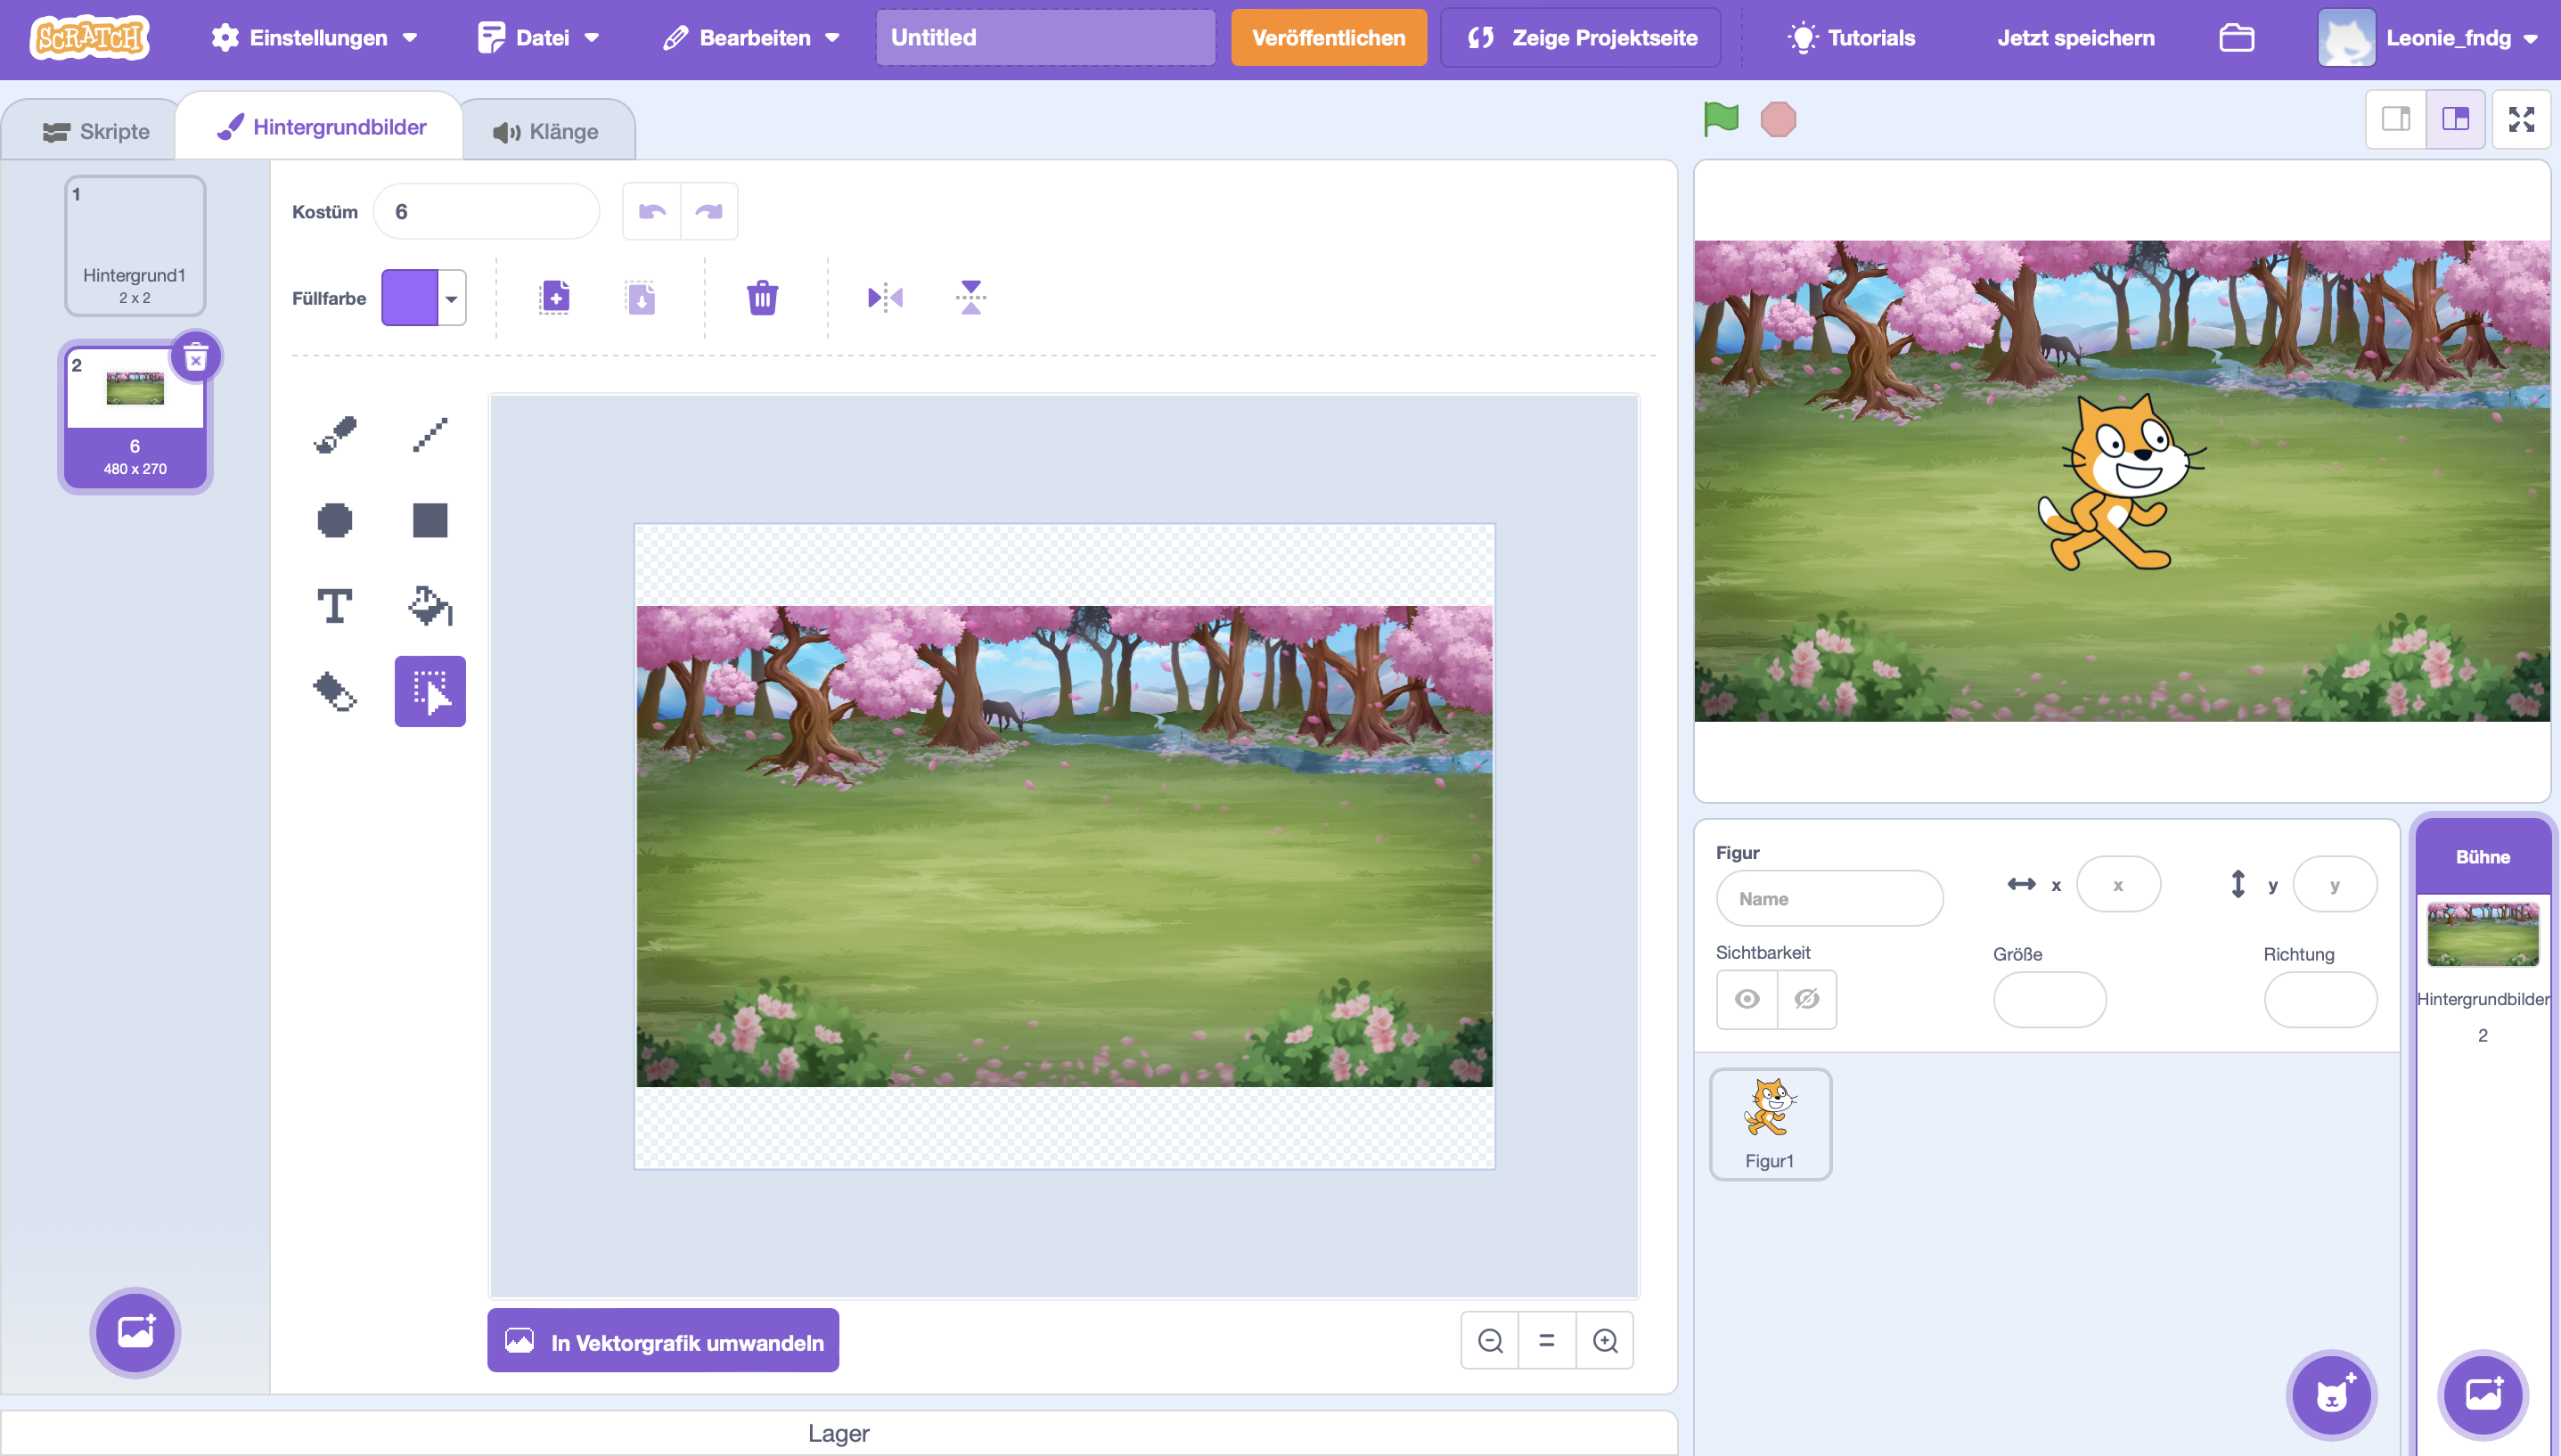
\includegraphics[width=0.8\textwidth, height=9cm]{StartBildschirmHZ.png}
    \vspace{1cm}

    
    \TextDesign{
    Wenn du dir die Vorschau (das kleinere rechte Bild) genauer ansiehst wirst du merken das wir oben und unten einen weißen Rand haben. Das wollen wir natürlich nicht deshalb müssen wir das Bild zurecht schneiden. Links auf deinen Bildschirm kannst du dein Hintergrundbild bearbeiten. Hier siehst du das aktuell lila Zeichen mit dem Pfeil. Wenn du drauf klickst kannst du sachen ausschneiden und dann vergrößern oder verkleinern. Klicke einmal auf das Zeichen und dann klicke mit deiner Maus (oder Mausped) auf die Linke obere Ecke und halte die Maus Taste, hier wirst du sehene das jetzt ein strichliertes Viereck entsteht wenn du den Zeiger bewegs. Ziehe deshalb deinen Zeiger an die rechte unter Ecke so das das ganze Bild makiert ist. 
    }

       \ImageAndText{Zurechtschneiden.png}{
  Wenn es jetzt so aussieht hast es richtig gemacht und kannst es jetzt an den blauen ecken vergrößern bis kein weißer Rand mehr da ist. Du kannst es natürlich auch mit den oberen und unteren Punkten vergrößern und verkleinern dadurch verziehst du aber das Bild. 
    }{0.6}{0.3}{12}{24}
    
     \vspace{0.5cm}
    
    \SectionDesign{subsection}{18}{24}{\textbf{Figuren festlegen und plazieren}}
\vspace{0.5cm}


\TextDesign{
Jetzt haben wir unser Hintergrund Bild. Aber da fehlt doch noch was oder? Genau, unsere Figuren! Davon brauchen wir nur drei unsere Bälle oder Bubbles, ein Figur was mit dem Benutzer agiert und natürlich  die Gefäße für die Bubbles. Ich werde dir gleich zeigen wie du diese hinzufügst ;) Hier siehst du unsere FIguren was wir brauchen: 
} 
\vspace{0.5cm}

 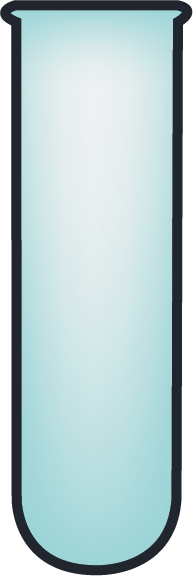
\includegraphics[width=0.10\textwidth, height=4cm]{Cup.png}
  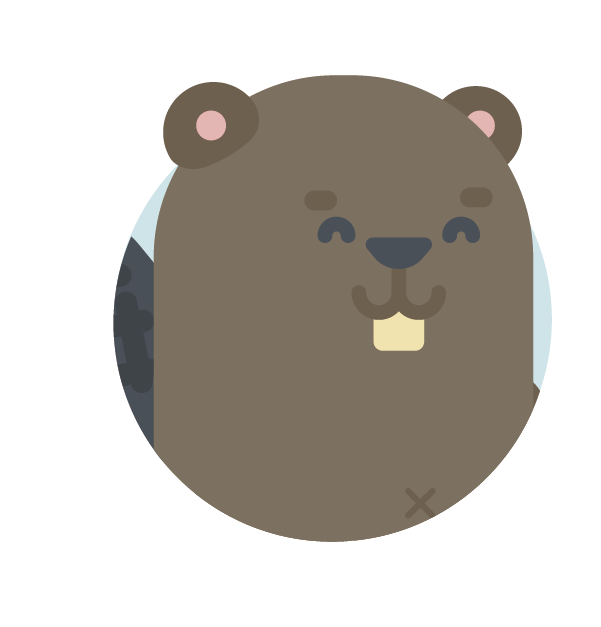
\includegraphics[width=0.25\textwidth, height=4cm]{Bieber.png}
   
\includegraphics[width=0.20\textwidth, height=3.5cm]{PinkerBall.png}

\vspace{0.5cm}

\TextAndImage{
   Als erstes müssen wir die standart Figur Figur löschen weil diese brauchen wir nicht, dafür musst du nur unten auf das kästchen mit der Figur klicken und auf das Mülleimer Symbol drücken dann wird die Figur sofort  gelöscht
    }{StandartFigurLöschen.png}{0.5}{0.2}{11}{16}

\vspace{0.5cm}

\TextAndImage{
   Jetzt müssen wir unsere Figuren hinzufügen. Das geht so ähnlich wie bei unseren Hintergrund wir müssen nur auf ein anderes Zeichen klicken, dieses befindet sich genuaso in der rechten unteren Hälfte unseres bildschirmes und ist links neben den Hintergrundzeichen. Wie du auf dem Bild erkennen kannst müssen wir wider auf das Zeichen mit dem Pfeil drücken um unsere Figuren zuerst hochzuladen. Das kannst du jetzt mal mit allen drei Figuren selber probieren. 
    }{FigurHochladen.png}{0.5}{0.2}{11}{16}

\vspace{0.5cm}

\TextAndImage{
  Wenn du es richtig gemacht hast müsste als erstes mal so aussehen. Keine Sorge wir werden unsere Figuren noch schön plazieren und richten;) Damit fangen wir auch gleich im nächsten Schritt an! 
    }{FigurenAmAnfang.png}{0.5}{0.2}{11}{16}
\vspace{0.5cm}

\TextDesign{
Um deinen Figuren einen Platz zu zu weisen und die größe von ihnen zu verändern benuzten wir die Toolbar: 
}

\vspace{0.5cm}

  \ImageAndText{Toolbar.png}{
    Bei "Figur" kannst du deiner Figur einen Namen geben oder sie umbennen. Das machen wir natürlich das wir am Ende eine gute übersicht haben! "Character6" ändern wir auf Bieber, "game Cup" auf Cup oder Behälter und "game Ball Pink" ändern wir nur auf Ball oder Bubble. Bei x und y können wir mit Koordinaten die Position festlegen hier haben wir für Bieber -> x = -190, y = 50; Cup/Behälter-> x = -10, y = 0 und für Ball/Bubble-> x = 74, y = 62 festgelegt. Als letztes kommen wir zu der Größe von unseren Figuren hierfür legst du für den Bieber = 40, Ball/Bubble = 25 und für unseren Cup/Behälter = 65 fest. 
    }{0.6}{0.75}{11}{16}

    \vspace{0.5cm}

    \TextAndImage{
  Wenn es ca. so aussieht hast du alles richtig gemacht:) BRAVO!!!
   Jetzt müssen wir nur noch eine Sache bei unseren Ball ändern unzwar braucht dieser verschiedene Kostüme warum wirst du später im Code erfahren }{RichtigAngelegt.png}{0.5}{0.2}{11}{16}

\vspace{0.5cm}
 
\ImageAndText{Kostüm.png}{
   Hierfür müssen wir auf unseren Ball klicken und auf Kostüme gehen das ist Links Oben in der Mitte. Das hinzufügen von Kostümen funktioniert genau gleich wie das hinzufügen von figuren. Das kannst du jetzt mal selber ausprobieren ich bin sicher du schaffst das! 
    }{0.4}{0.75}{11}{16}
    %NEWPAGE 
\newpage

\vspace{0.5cm}
\TextAndImage{
   Als erstes bekommst du hier eine Liste mit Variablen, du brauchst nur eine Liste namens Gefäße 
    }{Variablen.png}{0.5}{0.2}{11}{16}


\SectionDesign{subsection}{18}{24}{\textbf{Bieber Code}}

\vspace{0.5cm}

\TextAndImage{
   Wir fangen an mit unseren Gefäßen für die Bälle. Der erste Block gibt nur an das das alles ausgeführt werden soll wenn die Fahne angeklickt wird. Der zweite Lilane Block ist dafür da das die Gefäße nicht vor den Bällen sind und sie verdecken. Mit den zwei blauen Blöcken werden x und y festgelegt das die Figur immer am Anfang genau auf der Position ist und man sie nicht beliebig verschieben kann. Hier haben wir in Orange eine Variable diesew Sätzen wir auf null das unser erster Behälter auf der Position bleibt wo er ist. Danach klonen wir den Behälter 2 mal weil wir insgesamt drei Behälter haben wollen hier ändern wir auch die Position um 1 damit die nächsten Behählter nicht die gleiche Position wie der erste haben. Darunter haben wir noch einen kleinen Block dieser wird ausgeführt wenn der Klone erstellt wird und gibt ihm mit der Formel den richtigen Platz. Diese kannst du einfach nachbauen. 
    }{CupBlöcke.png}{0.5}{0.5}{11}{16}

    
    \newpage
    \vspace{0.5cm}
    
    \SectionDesign{subsection}{18}{24}{\textbf{Bälle erstellen und Gefäße füllen}}

   



    \vspace{0.5cm}

    \TextAndImage{
  Du wirst ganz viele eigene Blöcke in dieser Übung brauchen. Falls du nicht weist wie man Blöcke erstellt kommt hier eine Anleitung dazu ;) Wenn du in deiner BlockListe gaaannz nach unten gehst findest du einen roten Bereich mit neuer Block dort klickst du drauf. Mache unten bei "Ohne Bildschirmaktuallisierung laufen lassen" ein Häckchen hin. Wir werden bei dieser Übung erstmals auch nur zusätzlich eingabefelder dazu brauchen diese kannst du mit den Lila makierten Knopf hinzu fügen. Übrigends die Einteilung in Blöcken struckturiert das Programm in Textueller Programmierung wird das mit Methoden, Klassen und Funktionen gemacht. Ein großer Vorteil davon ist das man Blöcke immer wider verwenden kann wo man sonst villeiht den gleichen Code zweimal brauchen würde.
    }{NeuenBlockErstellen.png}{0.5}{0.5}{11}{16}

 \vspace{0.5cm}

    \TextDesign{
Wir fangen zuerst langsam an die zwei Blöcke auf den unteren Bildern musst du nur nachbauen die Kommentare veraten euch was sie machen;) Hiermit krigst du ein bischen übung mit Nachbauen und Blöcke verschachteln!
}

  \vspace{0.4cm}

    \includegraphics[width=0.6\textwidth, height=7cm]{ZeichenHinzufügen.png}
      \vspace{0.4cm}

    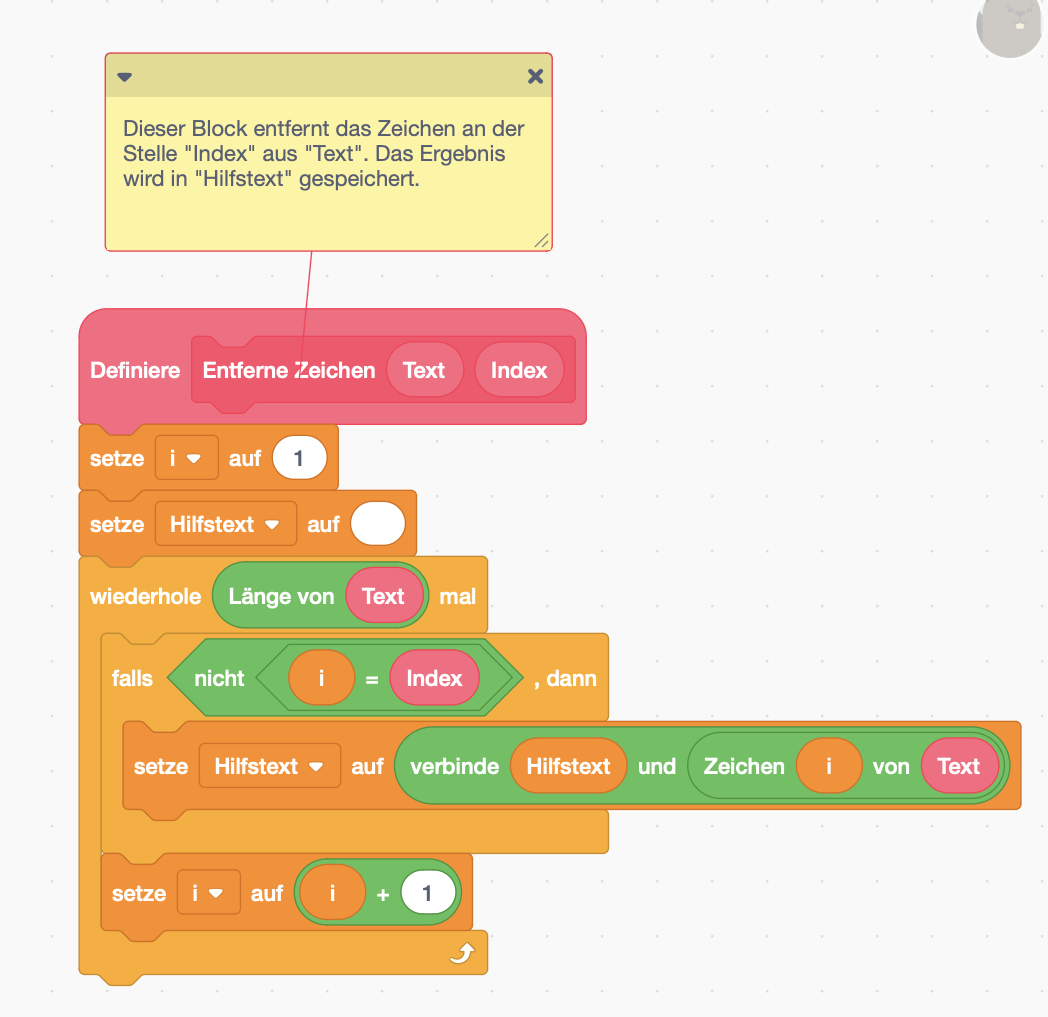
\includegraphics[width=0.6\textwidth, height=7cm]{ZeichenEntfernen.png}

        \TextAndImage{
  Für einen besseren überblick habe ich hier noch eine Liste mit den blöcken die du brauchen wirst (die Blöcke "Füge forne ein" und "entferne Zeichen" hast du jetzt natürlich schon;) )
    }{BlockListe.png}{0.5}{0.2}{11}{16}

    \vspace{0.5cm}

        \TextAndImage{
Da wir ja möchten das unser Benutzer mit dem Biber agieren kann müssen wir unseren Biber fragen lassen wohin der Benutzer die Kugel schieben möchte, dass machen wir mit diesen Block. Als erstes setzen wir von auf 0 in diese Variable wird die Antwort von dem Benutzer gespeichert. Dann widerholen wir eine schleife bis das von größer als 1 ist also bis wir eine antwort haben. mit dem blauen frage Block fragen wir, danach speichern wir in Antwort in unsere Variable "von". Mit den "Falls" block überprüfen wir ob der Benutzer auch wirklich nur Zahlen zwischen 1 und 3 eingegeben hat falls nicht wird eine fehlermeldung ausgegeben und von wider auf null gesetzt. In unseren "Sonst" haben wir nochmal ein falls eingebaut (keine Sorge bei Textueller Programmierung gibt es besser Möglichkeiten für so etwas) damit du dieses verstehst erkläre ich dir kurz das Grund konzept von unseren Programm. Unzwar haben wir eine Liste "Gefäße" in dieser ist für jedes Gefäß ein Eintrag mit Buchstaben wo jeder Buchstabe eine Farbe representiert. In diesen "Falls" wird überprüft ob das Gefäß von wo wir die Kugel nehmen möchten leer ist, wenn ja kommt eine Fehlermeldung und wir setztn von wider auf 0. Somit läuft die Schleife so lange bis wir eine gültige Antwort erhalten.
    }{FrageQuell.png}{0.5}{0.6}{11}{16}


           \TextAndImage{

    }{FrageQuell.png}{0.5}{0.6}{11}{16} 
\end{document}
